\subsection{Assembler}
\label{sec:assembler}
Since we decided to not support some of the RV32I instructions and we were not going to compile high level code, we decided to write our own custom assembler. So we came up with \textit{com.py}. It is not a compiler, despite the name, nor a full RV32I assembler, and doesn't claim to be. The main reason for its name is the fact that it ends in \textit{py}, and there you are the wordplay with its extension. Still, an assembler could be seen as a simple compiler for a low level language. 

\subsubsection{Features}
Here is a little perspective on the main feature of \textit{com.py}.
\begin{itemize}
   \item Most of the instructions from RV32I are supported, excluding:
   \begin{itemize}
      \item Environmental CALL (\texttt{ecall}) and BREAK (\texttt{ebreak}) instructions
      \item Synch thread (\texttt{fence}) and synch instruction \& data (\texttt{fence.i}) instructions
      \item Status register manipulation instructions (\texttt{csr*})
   \end{itemize}
   \item Most pseudo-instruction are supported, excluded the ones that have to be translated to more than one instruction and those related to the unsupported base instructions.
   \item All the instructions and pseudo-instructions are processed and assembled making heavy use of python dictionaries. This greatly simplifies the code and most important keeps the assembler modular. Adding a new instruction is normally as easy as introducing a new \texttt{[key]: [value]} couple to the dictionaries. 
   \item The output machine code can be provided both as ASCII binary file or ASCII hexadecimal file, so that they can be employed as source files for simulation.
   \item If requested, assembler can set-up a System Verilog file containing the simulation parameters, linking it to the assembled machine code. Then, a simulation script is launched in Modelsim. 
   \item Registers can be addressed by their architectural names (\texttt{x[n]}) or by their ABI (Application Binary Interface) names (e.g. \texttt{ra} or \texttt{sp}). 
   \item The offset field can be passed both as a standalone parameter (e.g \texttt{sw rs1, rs2, imm}) or as parenthesis prefix (e.g \texttt{sw rs2, imm(rs1)}). 
   \item Comments are introduced by character \texttt{\#} and are ignored.
   \item Very basic syntax error detection is provided.
   \item This is not meant to be a usage guide, so run \texttt{./com.py -h} for more help.
\end{itemize}

\subsubsection{How it works}
Figure \ref{fig:compy} shows a qualitative flow chart of the assembler. After opening the input file, the script reads one line at a time and remove comments. Pseudo-instructions are then converted to base ones and processed, while the canonical format (\texttt{instr\_name param1, param2, [param3]}) is retrieved. Then, all the instructions are processed the same way. The fields of the machine code that depends only on the type of instruction and the instruction name are processed first. After, the parameters like registers and immediate/offset fields are encoded based on the instruction type. Eventually, all the fields are printed on screen, joined together and appended to a ASCII binary output file with extension \texttt{.mc}. Since the assembler doesn't keep a copy of the entire code but processes one instruction at a time, memory usage is kept under control even when dealing with long pieces of assembly code. 

As soon as an error is encountered processing one line (i.e. one instruction) the user is warned by a message on screen and the assembler exits with a specific error code. This makes it possible to use this script inside other bash or python scripts. Errors are handled by means of python exception handling \texttt{try:... except:...} construct, that interprets these exceptions based on the assembling context instead of throwing generic python interpreter errors to the user. 

Eventually, if no error was encountered, a hexadecimal file with extension \texttt{.riscv} is generated starting from the binary one. If requested, the script proceeds linking the assembled code in a System Verilog test-bench configutation file and launches the simulation in Modelsim, running a \texttt{.tcl} script with the necessary commands to compile and simulate the entire design. Since this configuration file can also be used for other purposes, \textit{com.py} keeps a copy of the old version and restores it when Modelsim is quit. 

\begin{figure}[hbtp]
   \centering
   \includegraphics[scale=.7]{../common/ref/schematic/compy.pdf}
   \caption{\textit{com.py} flow chart}
   \label{fig:compy}
\end{figure}